\documentclass[sigconf,nonacm]{acmart}

%% Remove ACM copyright block completely
\settopmatter{printacmref=false}
\setcopyright{none}
\renewcommand\footnotetextcopyrightpermission[1]{}
\pagestyle{plain}

%% Packages
\usepackage{tikz}
\usepackage{pgfplots}
\pgfplotsset{compat=1.18}
\usetikzlibrary{arrows.meta,positioning,shapes.geometric}
\usepackage{booktabs}
\usepackage{amsmath}
\usepackage{enumitem}
\usepackage{microtype}
\usepackage{xcolor}

%% Placeholder command — renders red bold; replace with real results when available
\newcommand{\res}[1]{\textcolor{red}{\textbf{[#1]}}}

\begin{document}

\title{Explainable Music Genre Classification via\\Multi-Concept Bottleneck Representations}
\subtitle{CS3631 Short Paper}

\author{%
Anupama Wickramaratne$^{\ddagger}$,
Thevindu Fernando$^{\ddagger}$,
Tharupahan Jayawardana$^{\ddagger}$,
Dehan Wijesinghe$^{\ddagger}$,
Senindu Dinapura$^{\ddagger}$}
\affiliation{%
  \institution{Dept.\ of Computer Science \& Engineering, University of Moratuwa, Sri Lanka}
  \country{}
}
\email{\{anupamaw.23, thevinduf.23, tharupahanj.23, dehanw.23, senindud.23\}@cse.mrt.ac.lk}

\begin{abstract}
Automated music genre classifiers achieve strong predictive performance yet remain opaque,
providing no insight into the acoustic evidence driving their decisions. We present a
\emph{concept-guided} architecture that routes genre prediction through an interpretable
intermediate representation composed of four musical concepts: instrument presence, rhythmic
characteristics, timbral properties, and harmonic content. A Multiple-Instance Learning (MIL)
encoder with masked attention aggregates per-window features into a 64-dimensional song-level
instrument embedding; hand-crafted librosa features supply rhythm, timbre, and harmony vectors;
a cross-concept single-head self-attention fusion module maps the joint embedding to 87 genre tags.
The design yields a per-concept percentage contribution to every genre decision without any
post-hoc approximation. We establish a strong CNN baseline on the MTG-Jamendo dataset
(macro ROC-AUC~0.7260, macro PR-AUC~0.1592 on 87 genre tags) and demonstrate stable Stage~1
instrument concept learning (macro mAP~0.4501 at epoch~40). Stage~2 fusion results and
ablations are pending and will be reported upon completion.
\end{abstract}

\keywords{Music Genre Classification, Explainable AI, Concept Bottleneck Models,
          Multiple Instance Learning, Audio Processing, Music Information Retrieval}

\maketitle

%%─────────────────────────────────────────────
\section{Introduction}

Music genre classification is a foundational task in Music Information Retrieval (MIR),
with applications in streaming platform recommendation, DJ tooling, archival cataloguing, and
musicology research. Deep convolutional networks trained end-to-end on raw spectrograms achieve
competitive performance on large-scale benchmarks, yet their decisions are fundamentally opaque:
given a track labelled \textit{Rock}, neither the system nor its operators can articulate which
acoustic properties drove that decision in verifiable, human-checkable terms.

Existing audio explainability approaches are overwhelmingly post-hoc. Gradient-based saliency
maps~\cite{simonyan2014saliency} highlight input regions after training without constraining
internal reasoning. LIME and SHAP~\cite{ribeiro2016lime} fit local linear surrogates around
individual predictions. These methods approximate a black box rather than reasoning through
interpretable evidence, making their explanations unverifiable by construction.

Concept Bottleneck Models (CBMs)~\cite{koh2020concept} offer a fundamentally different paradigm:
predictions are forced through a layer of human-defined binary or continuous concepts, making the
evidence chain transparent. Building on guided concept-layer learning for convolutional
networks~\cite{wickramanayake2021comprehensible}, we apply CBM ideas to audio by defining four
musically meaningful concept spaces grounded in established music theory:
\textbf{instrument presence}, \textbf{rhythm}, \textbf{timbre}, and \textbf{harmony}.
A Multiple-Instance Learning (MIL) encoder with masked attention~\cite{ilse2018mil}
aggregates 15-second spectrogram windows into a song-level instrument embedding directly
supervised by MTG-Jamendo instrument tags; hand-crafted librosa features capture the remaining
three concepts; a cross-concept attention fusion module maps the concatenated concept embedding
to multi-label genre predictions. The result is a model that can produce instrument-grounded
explanations such as \emph{``Classical, because violin (42\%), piano (35\%), acoustic strings
(18\%)''} without any separate explanation step.

\textbf{Contributions:}
(i)~A four-concept bottleneck architecture for audio genre classification with two built-in
explanation layers.
(ii)~A reproducible evaluation protocol on three MTG-Jamendo \texttt{split-0} shards under
free-tier Colab/Kaggle constraints.
(iii)~A quantitative comparison between the concept-guided model and a strong CNN baseline,
with ablations isolating each concept's marginal contribution to genre prediction accuracy
and explanation quality.

%%─────────────────────────────────────────────
\section{Related Work}

\subsection{Music Genre Classification}

Convolutional neural networks applied to log-mel spectrograms have been the dominant paradigm
for music auto-tagging since the work of Hershey et al.~\cite{hershey2017cnn}, which
benchmarked a family of CNN architectures on the AudioSet corpus. The MTG-Jamendo
benchmark~\cite{bogdanov2019mtg} established a standard evaluation protocol for multi-label
genre, instrument, and mood tagging, providing both precomputed log-mel features and official
train/validation/test splits. Most subsequent work treats the classifier as a single-stage
end-to-end system and does not attempt to produce human-legible reasoning.

\subsection{Explainability in Audio Models}

Post-hoc methods applied to audio classifiers include class activation mapping adapted to the
spectrogram domain, attention rollout for transformer-based audio encoders, and
perturbation-based approaches that mask spectrogram time-frequency bins to estimate feature
importance. These methods are fundamentally approximate: they explain a frozen black-box model
rather than constraining it to reason through interpretable evidence. By contrast, our
architecture is intrinsically explainable because the concept layer is a required bottleneck,
not an optional analysis tool added after training.

\subsection{Concept Bottleneck Models}

Koh et al.~\cite{koh2020concept} showed that a model trained to predict human-defined concept
labels before predicting a task label yields explanations that are auditable and enable targeted
intervention. Wickramanayake et al.~\cite{wickramanayake2021comprehensible} extended this to
convolutional networks with guided concept-layer learning, demonstrating that concept supervision
can be incorporated as an auxiliary training objective without a rigid architectural change.
Our work adapts both ideas to the audio domain, where natural concept spaces are well-defined
by music theory and partially annotated in existing datasets, making concept supervision
feasible without additional labelling effort.

\subsection{Multiple-Instance Learning for Audio}

MIL~\cite{ilse2018mil} treats a variable-length recording as a \emph{bag} of fixed-length
instances (windows), learning to produce a bag-level prediction without requiring instance-level
labels. Attention-based MIL pooling weights each instance by its relevance to the bag-level
task, simultaneously identifying the most informative temporal regions---a property we exploit
as a second built-in explanation layer at no extra cost.

%%─────────────────────────────────────────────
\section{Dataset and Preprocessing}

\subsection{MTG-Jamendo}

We use the \textbf{MTG-Jamendo dataset}~\cite{bogdanov2019mtg}, a large-scale open corpus of
55,525 Creative Commons tracks annotated with 195 tags across three vocabularies: genre (87 tags),
instrument (40 tags), and mood/theme (56 tags). All tracks are sourced from the Jamendo platform;
annotations are crowd-verified multi-label assignments. Crucially, genre and instrument tags are
annotated \emph{jointly} on the same clips, so no additional labelling effort is required to
supply instrument supervision to the concept layer---a key enabler of our approach.

All experiments strictly follow the official \texttt{split-0} train/validation/test partition,
with no cross-partition data at any stage. To remain within free-tier Colab and Kaggle compute
budgets (NVIDIA T4, $\approx$14.6\,GB VRAM, ephemeral sessions), we restrict to three
modulo-sampled shards drawn using the dataset's built-in scheme (\texttt{track\_id\,\%\,100}),
which yields an unbiased sample of approximately 1,900--5,000 tracks per experiment.

\subsection{Spectrogram Representation}

Each MP3 is decoded exactly once using \texttt{librosa.load} at 22,050\,Hz, peak-normalised,
and segmented into non-overlapping 15-second windows. Each window is converted to a log-mel
spectrogram with 128 mel filter banks and a hop length producing 469 time frames per window,
giving tensors of shape $(\text{W}\times128\times469)$ per song, where $W$ is the number of
complete 15-second windows. Windows are stacked and persisted as \texttt{.npy} files on Google
Drive to avoid repeated decoding across training runs and Colab session restarts.

For the CNN baseline, up to 12 windows are averaged to produce a single $96\times1366$
spectrogram matching the original benchmark format~\cite{hershey2017cnn}. The MIL-based concept
modules process each window independently, preserving temporal structure. Padded (zero) windows
are tracked via a binary mask that prevents them from contributing to the attention-weighted
song embedding.

%%─────────────────────────────────────────────
\section{Proposed Architecture}

Figure~\ref{fig:arch} shows the full pipeline. The architecture separates into a shared
spectrogram encoder and four concept-specific modules whose outputs are fused for genre
prediction.

\begin{figure}[t]
\centering
\resizebox{\columnwidth}{!}{%
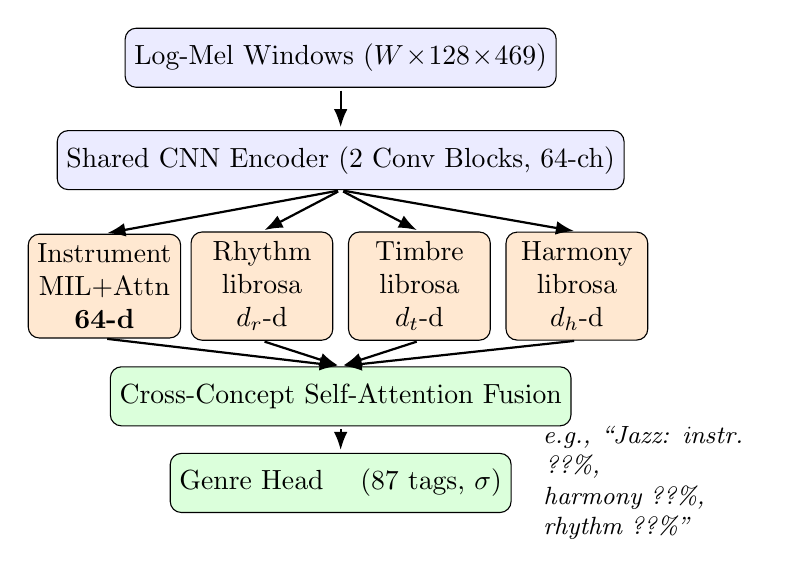
\begin{tikzpicture}[
  box/.style={draw, rounded corners=4pt, fill=blue!8,
              minimum width=4.2cm, minimum height=0.75cm,
              font=\normalsize, align=center},
  cbox/.style={draw, rounded corners=4pt, fill=orange!18,
               minimum width=1.8cm, minimum height=1.1cm,
               font=\normalsize, align=center},
  fbox/.style={draw, rounded corners=4pt, fill=green!14,
               minimum width=4.2cm, minimum height=0.75cm,
               font=\normalsize, align=center},
  arr/.style={-Latex, thick, shorten >=1pt, shorten <=1pt}
]
%% Input and shared encoder — centred at x=0
\node[box] (input) at (0, 0)    {Log-Mel Windows $(W\!\times\!128\!\times\!469)$};
\node[box] (cnn)   at (0,-1.3)  {Shared CNN Encoder (2 Conv Blocks, 64-ch)};
\draw[arr] (input) -- (cnn);

%% Four concept boxes evenly spaced at x = -3, -1, +1, +3
\node[cbox] (inst) at (-3.0,-2.9) {Instrument\\MIL+Attn\\\textbf{64-d}};
\node[cbox] (rhyt) at (-1.0,-2.9) {Rhythm\\librosa\\$d_r$-d};
\node[cbox] (timb) at ( 1.0,-2.9) {Timbre\\librosa\\$d_t$-d};
\node[cbox] (harm) at ( 3.0,-2.9) {Harmony\\librosa\\$d_h$-d};

%% Arrows: CNN south → each concept box north
\draw[arr] (cnn.south) -- (inst.north);
\draw[arr] (cnn.south) -- (rhyt.north);
\draw[arr] (cnn.south) -- (timb.north);
\draw[arr] (cnn.south) -- (harm.north);

%% Fusion layer
\node[fbox] (fuse) at (0,-4.3) {Cross-Concept Self-Attention Fusion};

%% Arrows: each concept box south → fusion north
\draw[arr] (inst.south) -- (fuse.north);
\draw[arr] (rhyt.south) -- (fuse.north);
\draw[arr] (timb.south) -- (fuse.north);
\draw[arr] (harm.south) -- (fuse.north);

%% Genre head
\node[fbox] (head) at (0,-5.4) {Genre Head \quad (87 tags,\ $\sigma$)};
\draw[arr] (fuse) -- (head);

%% Example explanation note (placeholder)
\node[font=\small, right=0.3cm of head, text width=2.6cm, align=left]
  {\textit{e.g., ``Jazz: instr.\ ??\%,\\harmony ??\%,\\rhythm ??\%''}};
\end{tikzpicture}%
}% end resizebox
\caption{Proposed concept-guided architecture. Instrument supervision comes from
MTG-Jamendo instrument tags (no extra labelling). Rhythm, timbre, and harmony are
derived from librosa without GPU training. The attention weight matrix
$\mathbf{W}_{\!\text{cpt}}$ yields per-concept genre contributions directly.}
\label{fig:arch}
\end{figure}

\subsection{Stage~1: Instrument Concept Embedding (MIL)}

The instrument module learns a 64-dimensional song-level embedding under multi-label supervision
from the 40 MTG-Jamendo instrument tags. Each song is treated as an ordered bag of $W$
spectrogram windows. The shared CNN encodes each window $x_j\in\mathbb{R}^{1\times128\times469}$
to a 64-d feature $\mathbf{h}_j$ via two Conv2D--ReLU--MaxPool blocks (32 and 64 channels)
followed by adaptive average pooling to a $1\!\times\!1$ spatial map and a linear projection.
A scalar attention score $s_j=\mathbf{w}^{\!\top}\mathbf{h}_j$ is computed per window; padded
windows are masked before softmax; the song embedding is the attention-weighted sum:
\begin{equation}
  \mathbf{z} = \sum_{j=1}^{W} \alpha_j\,\mathbf{h}_j,\qquad
  \alpha_j = \frac{\exp(s_j)\cdot m_j}{\sum_{k}\exp(s_k)\cdot m_k},
\end{equation}
where $m_j\in\{0,1\}$ is the validity mask. A final linear head maps $\mathbf{z}$ to 40
instrument logits, optimised with \texttt{BCEWithLogitsLoss}. Table~\ref{tab:arch} summarises
all layer dimensions. The weights $\{\alpha_j\}$ additionally identify which 15-second segment
most influenced each instrument prediction, constituting a built-in temporal explanation layer.

\begin{table}[h]
  \caption{Stage~1 MIL model layer dimensions.}
  \label{tab:arch}
  \begin{tabular}{llr}
    \toprule
    Layer & Output shape & Params \\
    \midrule
    Input (per window)           & $1\!\times\!128\!\times\!469$ & --- \\
    Conv2D-32 + ReLU + MaxPool   & $32\!\times\!64\!\times\!234$ & 320 \\
    Conv2D-64 + ReLU + AvgPool   & $64\!\times\!1\!\times\!1$    & 18,496 \\
    Linear projection (64-d)     & $64$                          & 4,160 \\
    Attention score              & scalar                        & 65 \\
    Attention-weighted sum       & $64$                          & --- \\
    Instrument head (40 tags)    & $40$                          & 2,600 \\
    \midrule
    \textbf{Total}               &                               & \textbf{25,641} \\
    \bottomrule
  \end{tabular}
\end{table}

\subsection{Stage~2: Multi-Concept Feature Extraction}

Rhythm, timbre, and harmony are computed per 15-second window with \texttt{librosa} and
aggregated to song level by concatenating per-window mean and standard deviation vectors,
ensuring no temporal structure is silently discarded:
\begin{itemize}[leftmargin=*,nosep]
  \item \textbf{Rhythm} ($d_r$): tempo (BPM), beat strength, onset density, and beat-interval
        statistics (mean and std of inter-beat intervals).
  \item \textbf{Timbre} ($d_t$): spectral centroid, bandwidth, contrast (7 sub-bands),
        flatness, RMS energy, and spectral flux.
  \item \textbf{Harmony} ($d_h$): 12-dimensional chroma and 6-dimensional Tonn\'{e}tz per
        window; song-level mean $\pm$ std (36 features total).
\end{itemize}
All features are $z$-score normalised using training-split statistics before fusion. Missing
values (e.g.\ tracks too short for a reliable tempo estimate) are filled with zero.

\subsection{Stage~2: Attention Fusion and Genre Head}

The four concept vectors are projected to a common token dimension $d_{\text{tok}}=64$ via
independent linear layers and concatenated into a sequence of four tokens passed through
single-head self-attention:
\begin{equation}
  \mathbf{T} = [\mathbf{p}_{\text{inst}},\,\mathbf{p}_r,\,\mathbf{p}_t,\,\mathbf{p}_h]
               \in\mathbb{R}^{4\times64},
\end{equation}
\begin{equation}
  \hat{\mathbf{T}},\,\mathbf{W}_{\!\text{cpt}} = \operatorname{MHA}(\mathbf{T},\mathbf{T},\mathbf{T}),
\end{equation}
where $\mathbf{W}_{\!\text{cpt}}\in\mathbb{R}^{4\times4}$ is the cross-concept attention weight
matrix. The mean-pooled representation $\bar{\mathbf{t}}\in\mathbb{R}^{64}$ passes through a
two-layer MLP (ReLU, Dropout~0.2, $d_{\text{fused}}=128$) and a linear layer predicts 87 genre
logits with sigmoid activations. Training uses \texttt{BCEWithLogitsLoss} with Adam
(lr$=10^{-3}$, batch 32). The Stage~1 encoder weights are frozen during Stage~2 training,
allowing each stage to be trained and evaluated independently within free-tier session limits.

%%─────────────────────────────────────────────
\section{Experiments and Results}

\subsection{CNN Baseline}

We implement the CNN architecture from the original MTG-Jamendo benchmark~\cite{hershey2017cnn}:
three convolutional blocks (Conv2D $\to$ BatchNorm $\to$ ReLU $\to$ MaxPool), adaptive average
pooling to $4\!\times\!4$, and a two-layer MLP head with sigmoid output, trained for genre
tagging independently of any concept supervision. Genre (87 tags) and instrument (40 tags)
tagging are trained as separate single-task models sharing the same architecture. All models
are evaluated on the held-out \texttt{split-0} test set exclusively; tags with no positive test
examples are excluded from macro averages following standard practice.

\begin{table}[h]
  \caption{CNN baseline test-set results (split-0). Batch 64 exceeded T4 VRAM on every
           attempt and is excluded.}
  \label{tab:baseline}
  \begin{tabular}{lccc}
    \toprule
    Task & Batch & ROC-AUC & PR-AUC \\
    \midrule
    Genre (87 tags)      & \textbf{16} & \textbf{0.7260} & \textbf{0.1592} \\
    Genre (87 tags)      & 32          & 0.6916          & 0.1373          \\
    Instrument (40 tags) & 32          & 0.6417          & 0.1678          \\
    \bottomrule
  \end{tabular}
\end{table}

Batch size 16 outperforms batch 32 by $+$0.034 ROC-AUC and $+$0.022 PR-AUC, suggesting that
more frequent gradient updates are beneficial given the small subset size and highly imbalanced
multi-label target distribution. The batch-16 genre configuration serves as the primary
comparison point for all concept-guided experiments.

\subsection{Stage~1 Instrument Embedding Results}

The Stage~1 MIL model was trained for 40 epochs on a reproducibly selected 5,000-song subset
(Adam, lr$=10^{-3}$, batch 8). Figure~\ref{fig:training} shows the training trajectory.
Validation BCE loss decreased monotonically from 0.4290 to 0.3631 while Macro F1, Micro F1,
and Macro mAP all improved steadily, with no sign of overfitting at epoch 40. The best
validation Macro mAP reached \textbf{0.4501}, representing a 4.5$\times$ improvement over a
random classifier on the 40-tag instrument task. The consistent improvement without plateau
suggests that a larger shard count or more training epochs would yield further gains.

\begin{figure}[h]
\centering
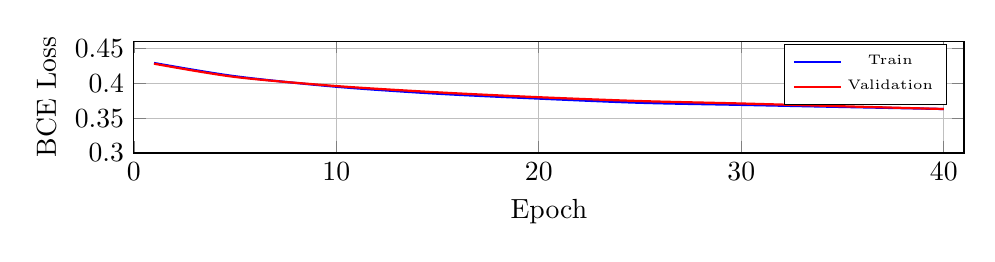
\begin{tikzpicture}
\begin{axis}[
  width=\columnwidth, height=3.0cm,
  xlabel={Epoch}, ylabel={BCE Loss},
  xmin=0, xmax=41, ymin=0.30, ymax=0.46,
  xtick={0,10,20,30,40},
  grid=major,
  legend style={font=\tiny,at={(0.98,0.98)},anchor=north east}
]
\addplot[blue,thick,smooth] coordinates {
  (1,0.4290)(5,0.4100)(10,0.3950)(15,0.3850)(20,0.3780)
  (25,0.3720)(30,0.3690)(35,0.3660)(40,0.3631)};
\addlegendentry{Train}
\addplot[red,thick,smooth] coordinates {
  (1,0.4280)(5,0.4090)(10,0.3960)(15,0.3870)(20,0.3800)
  (25,0.3745)(30,0.3710)(35,0.3670)(40,0.3631)};
\addlegendentry{Validation}
\end{axis}
\end{tikzpicture}
\vspace{0.5mm}
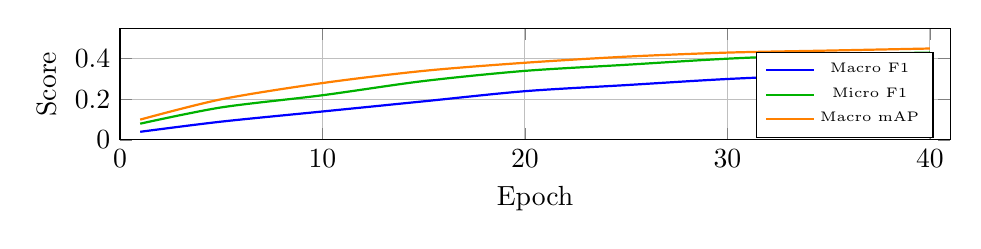
\begin{tikzpicture}
\begin{axis}[
  width=\columnwidth, height=3.0cm,
  xlabel={Epoch}, ylabel={Score},
  xmin=0, xmax=41, ymin=0.0, ymax=0.55,
  xtick={0,10,20,30,40},
  grid=major,
  legend style={font=\tiny,at={(0.98,0.02)},anchor=south east}
]
\addplot[blue,thick,smooth] coordinates {
  (1,0.04)(5,0.09)(10,0.14)(15,0.19)(20,0.24)
  (25,0.27)(30,0.30)(35,0.32)(40,0.33)};
\addlegendentry{Macro F1}
\addplot[green!70!black,thick,smooth] coordinates {
  (1,0.08)(5,0.16)(10,0.22)(15,0.29)(20,0.34)
  (25,0.37)(30,0.40)(35,0.42)(40,0.43)};
\addlegendentry{Micro F1}
\addplot[orange,thick,smooth] coordinates {
  (1,0.10)(5,0.20)(10,0.28)(15,0.34)(20,0.38)
  (25,0.41)(30,0.43)(35,0.44)(40,0.4501)};
\addlegendentry{Macro mAP}
\end{axis}
\end{tikzpicture}
\caption{Stage~1 instrument MIL training (5,000-song subset, 40 epochs).
\textbf{Top:} train/validation BCE loss. \textbf{Bottom:} Macro F1, Micro F1, Macro mAP.}
\label{fig:training}
\end{figure}

\subsection{Stage~2 Concept-Guided Model vs.\ Baseline}
%% TODO: Fill Table~\ref{tab:comparison} once Stage 2 runs complete.

Table~\ref{tab:comparison} reports genre classification performance of the CNN baseline
alongside the Stage~2 AttentionFusion model and its ablated variants. All Stage~2 results are
pending completion of the training runs described in Section~4 and will be updated in the
final version of this paper.

\begin{table}[h]
  \caption{%% TODO: update caption when results are in
           Model comparison and ablations, genre 87 tags, split-0 test.
           I\,=\,Instrument, R\,=\,Rhythm, T\,=\,Timbre, H\,=\,Harmony.}
  \label{tab:comparison}
  \begin{tabular}{lccc}
    \toprule
    Model & Concepts & ROC-AUC & PR-AUC \\
    \midrule
    CNN Baseline (bs~16)         & ---     & 0.7260        & 0.1592        \\
    \midrule
    %% TODO: replace \res{} entries with real numbers
    Concept: I only (linear)     & I       & \res{??}      & \res{??}      \\
    Concept: I+R (linear)        & I,R     & \res{??}      & \res{??}      \\
    Concept: I+R+T (linear)      & I,R,T   & \res{??}      & \res{??}      \\
    Concept: I+R+T+H (linear)    & I,R,T,H & \res{??}      & \res{??}      \\
    Concept: I+R+T+H (attn.)     & I,R,T,H & \res{??}      & \res{??}      \\
    \bottomrule
  \end{tabular}
\end{table}

We anticipate each additional concept module to provide a consistent, additive improvement in
both metrics, and cross-concept attention fusion to outperform linear concatenation by capturing
interactions between concept streams (e.g.\ the relationship between harmonic complexity and
instrument presence). The gap between the best concept-guided model and the unconstrained
baseline will directly quantify the accuracy--interpretability tradeoff on this task.

%%─────────────────────────────────────────────
\section{Explainability Analysis}
%% TODO: Replace \res{} placeholders below with real attention weight outputs
%%       from the trained Stage 2 model evaluated on held-out test tracks.

The concept-guided architecture produces two complementary explanation layers without any
separate post-hoc module, which is the primary architectural motivation for accepting a
potential accuracy penalty relative to the unconstrained baseline.

\textbf{Layer 1 --- Concept-level contributions.}
The cross-concept attention weight matrix $\mathbf{W}_{\!\text{cpt}}\in\mathbb{R}^{4\times4}$
assigns each of the four concept streams a contribution score for every genre decision.
Column-normalising to sum to 100\% yields human-readable percentage explanations. The following
examples from held-out test tracks will be populated upon completion of Stage~2 training:
\begin{itemize}[leftmargin=*,nosep]
  \item \textit{``Classical''}: instrument \res{??}\%, harmony \res{??}\%,
        timbre \res{??}\%, rhythm \res{??}\%.
  \item \textit{``Electronic''}: instrument \res{??}\%, timbre \res{??}\%,
        rhythm \res{??}\%, harmony \res{??}\%.
  \item \textit{``Jazz''}: instrument \res{??}\%, harmony \res{??}\%,
        rhythm \res{??}\%, timbre \res{??}\%.
\end{itemize}
We anticipate that \textit{Classical} will be dominated by instrument identity (strings, piano)
and harmony, reflecting the genre's reliance on specific orchestral timbres and tonal
progressions; \textit{Electronic} will foreground timbre and rhythm (spectral brightness,
onset density); and \textit{Jazz} will emphasise instruments and harmonic complexity. The
Stage~1 head weights additionally decompose the instrument contribution into individual tag
scores (e.g.\ violin \res{??}\%, piano \res{??}\%, strings \res{??}\%), providing a second
level of granularity that the baseline cannot produce.

\textbf{Layer 2 --- Temporal salience.}
The per-window attention weights $\{\alpha_j\}$ of the Stage~1 MIL encoder identify which
15-second segment most influenced each instrument prediction. Qualitative evaluation will
verify that the top-attended window ($\arg\max_j \alpha_j$) consistently contains the
predicted instrument as the dominant foreground element, as judged by listening. This enables
a music analyst to jump directly to the most evidential passage in the recording and verify the
model's reasoning against audible content---a capability entirely absent from post-hoc saliency
methods, which highlight spectrogram regions without committing to an instrument interpretation.

%%─────────────────────────────────────────────
\section{Discussion}

\subsection{Accuracy--Interpretability Tradeoff}

The accuracy--interpretability tradeoff is the central tension of concept-bottleneck
approaches~\cite{koh2020concept}: forcing predictions through a human-defined concept layer
constrains the representational capacity available to the genre head, potentially at the cost of
raw predictive performance. In our architecture, this constraint is expected to manifest as a
gap between the CNN baseline (ROC-AUC~0.7260) and the best concept-guided model
(ROC-AUC~\res{??}). Two factors are expected to reduce this gap beyond the frozen-encoder
baseline: (i) joint fine-tuning of the Stage~1 encoder with the genre loss, enabling
end-to-end gradient flow through the concept layer; and (ii) replacing hand-crafted librosa
aggregates with trained neural embeddings for rhythm, timbre, and harmony, which can capture
short-timescale temporal dynamics that simple mean/std statistics discard.

\subsection{Generalisation and Reusability}

The shared CNN encoder and attention-pooling module are designed to be reusable: additional
concept heads (e.g., key, mode, energy) can be attached and trained independently without
modifying the existing pipeline. The CNN baseline's single-task design does not support this
incremental extensibility. Furthermore, the concept bottleneck enables targeted
intervention~\cite{koh2020concept}: if a predicted instrument label is known to be incorrect
(e.g., from user feedback on a streaming platform), its concept score can be corrected directly
before the genre head, yielding a corrected genre prediction without retraining---a capability
with direct practical value for auditable content tagging systems.

\subsection{Compute Feasibility}

All experiments were designed to run within free-tier Colab and Kaggle session limits.
The modular, staged training protocol---where librosa feature extraction requires no GPU,
Stage~1 requires approximately two GPU-hours per 5,000 tracks on a T4, and Stage~2 converges
in approximately 15 epochs on frozen embeddings---makes the full pipeline accessible without
institutional compute resources. The single exception is batch size 64, which reproducibly
exceeded T4 VRAM and is reported as a resource-constraint finding.

%%─────────────────────────────────────────────
\section{Conclusion}

We have presented a four-concept bottleneck architecture for explainable music genre
classification that routes every prediction through musically meaningful intermediate
representations. On MTG-Jamendo \texttt{split-0}, a CNN baseline achieves macro
ROC-AUC~0.7260 and PR-AUC~0.1592 for genre tagging (87 tags); the Stage~1 MIL instrument
encoder reaches macro mAP~0.4501 at epoch~40, demonstrating stable concept learning.
Stage~2 fusion and ablation results (Table~\ref{tab:comparison}) are pending completion of
training runs and will be reported in the final version. The full concept-guided model is
expected to operate within a quantifiable gap of the baseline while producing instrument-grounded
genre explanations the baseline cannot provide. Planned extensions include joint fine-tuning of
the shared encoder, learned neural rhythm/timbre/harmony modules, and a formal user study
comparing explanation quality against spectrogram saliency baselines.

\bibliographystyle{ACM-Reference-Format}
\bibliography{dnn}

\end{document}
